\chapter{Generador síncrono.}

	\section{Generalidades.}
		Los generadores síncronos o alternadores trifásicos autoexcitados en corriente continua que se usan en las centrales eléctricas se diferencian en función del número de vueltas de sus máquinas motrices.
		
		
		Velocidad síncrona en régimen permanente:
		
		\[n = \dfrac{60\cdot f}{p}\,[rpm]\]
		
		Donde $f$ es la frecuencia industrial y $p$ el número de pares de polos.
		
		
		\subsection{Aplicaciones de la máquina síncrona.}
			\begin{itemize}
				\item \textbf{Como generador:}
					\begin{itemize}
						\item Suministro de potencia a la red.
						\item Suministro de emergencia (hospitales, centros comerciales...).
						\item Instalaciones aisladas (redes rurales).
					\end{itemize}
					
				\item \textbf{Como motor:}
					\begin{itemize}
						\item Aplicaciones con velocidad constante (bombeo en centrales hidráulicas reversibles).
						\item Compensador síncrono en centrales (regulación del factor de potencia).
					\end{itemize}
			\end{itemize}
			
		\subsection{Aspectos constructivos.}
			\begin{itemize}
				\item \textbf{Inducido:}
					\begin{itemize}
						\item Se alimenta con corriente alterna trifásica.
						\item Con expansiones polares y devanado concentrado.
						\item Cilíndrico y con devanado concentrado o distribuido.
						\item Generalmente conectado en Y, con el neutro puesto a tierra.
					\end{itemize}
				
				\item \textbf{Inductor:}
					\begin{itemize}
						\item Se alimenta en corriente continua mediante anillos rozantes.
						\item \textit{Polos salientes:} devanado concentrado con devanado amortiguador (barras de cobre cortocircuitadas) para reducir oscilaciones pendulares y facilitar el arranque.
						\item \textit{Polos lisos o rotor cilíndrico:} devanado distribuido en ranuras.
					\end{itemize}
			\end{itemize}
				
			\begin{table}[H]
				\centering
				\renewcommand{\arraystretch}{1.1}
				\begin{tabular}{c|ccc}
					\textbf{Tamaño} & \textbf{Potencia} & \textbf{Inductor} & \textbf{Inducido} \\
					\hline
					Pequeñas & $<10\,kV\!A$ & Estátor, expansiones polares & Rotor, anillos rozantes \\
					Grandes & De $10\,kV\!A$ hasta $1500\,MV\!A$ & Rotor, sin anillos rozantes & Estátor\\
				\end{tabular}
			\end{table}		
			
	\section{Particularidades según su emplazamiento.}
		\subsection{Alternadores de centrales hidroeléctricas.}
			\begin{itemize}
				\item Tienen \textbf{diámetros} de entre 5 y 7 metros y \textbf{longitudes} de entre 1 y 2 metros.
				\item \textbf{Potencias} en torno a $200\,MV\!A$.
				\item En las grandes centrales hidráulicas su \textbf{velocidad de sincronismo} es de entre 60 y 125 $rpm$.
				\item Son de \textbf{polos salientes}, con hasta \textbf{40 pares de polos}.
				\item Suelen ser de \textbf{eje vertical}, situándose el \textbf{alternador encima de la turbina}.
				\item Tienen un \textbf{devanado amortiguador}, que actúa de jaula de ardilla para poder arrancar como motor asíncrono.
			\end{itemize}
			    
		\subsection{Alternadores de centrales térmicas.}
			\begin{itemize}
				\item Tienen \textbf{diámetros} de entre 1 y 2 metros y \textbf{longitudes} de entre 10 y 12 metros.
				\item \textbf{Potencias} de hasta $1500\,MV\!A$.
				\item \textbf{Tensión de generación} de 6 a 30 $kV$.
					\begin{itemize}
						\item A más tensión menor es la sección de los conductores.
						\item Intervalo de regulación previsto del $\pm 5\%$.
						\item En generaodres de baja tensión ($U_N = 400\,V$) la potencia está limitada a $2\,MV\!A$.
					\end{itemize}	
				\item Su \textbf{velocidad de sincronismo} es de 1500 ó 3000 $rpm$.
				\item Son de \textbf{rotor cilíndrico} con bobinado de excitación distribuido.
				\item Son de \textbf{eje horizontal}.
				\item Limitaciones en la refrigeración, la resistencia de los materiales y el peso.
			\end{itemize}
			
	\section{Refrigeración en los generadores síncronos.}
		Los calentamientos habituales se deben a rozamientos mecánicos, pérdidas por efecto Joule en los devanados y pérdidas por histéresis magnética y corrientes de Foucault en los núcleos ferromagnéticos.
		
		
		El aislamiento de los bobinados está hecho a base de resinas sintéticas termoelásticas sin disolventes (\textit{Thermolastic}). Se deterioran con un exceso de temperatura. Deben tener alta rigidez dieléctrica, aislamiento elástico con buena resistencia mecánica y resistencia a la humedad.
		
		
		Una buena refrigeración permite aumentar la corriente del rotor, aumentando la eficiencia hasta un $\eta = 98.5\%$ a la potencia nominal. Se alcanzan densidades de corriente de hasta 250 $kA/m^2$ e inducciones de $1.2\,T$. Hoy en día se fabrican aislamientos del estator impregnados al vacío, que son más resistentes al envejecimiento y totalmente insensibles al aceite y agua.
		
		
		Las bobinas se trasponen por el sistema ROEBEL, para aminorar las pérdidas debido a un reparto desigual
		del flujo magnético.
			
		\subsection{Tipos de refrigeración en máquinas de gran potencia.}
			\begin{itemize}
				\item Refrigeración directa por aire hasta $40\,MV\!A$ (grupos turboalternadores industriales).
				\item Refrigeración por hidrógeno seco (la humedad disminuye la conductividad) $>100\,MV\!A$.
				\item Refrigeración directa por agua destilada.
				\item Refrigeración mixta por hidrógeno y agua destilada.
				\item Refrigeración con helio: gas inerte y no inflamable, pero volátil, más caro y escaso.
			\end{itemize}
			
		\subsection{Sistemas de refrigeración de las bobinas rotóricas y estatóricas.}
			Actualmente, se hace circular el fluido refrigerante en el mismo interior de los conductores, donde se produce el calor. De esta forma se mejora enormemente la transferencia de calor al fluido refrigerante, y disminuye el aumento de temperatura en el aislamiento de los conductores, prolongando su vida.
			
			
			En casi todos los generadores para centrales hidráulicas se emplea refrigeración mixta: por
			aire en el circuito del rotor y agua destilada en el circuito del estator.
			
			
			Para los turbogeneradores las refrigeraciones más empleadas para el circuito del estator son refrigeración por hidrógeno a 6 $bar$ y refrigeración por agua destilada.
			
		\subsection{Aspectos constructivos del rotor cilíndrico.}
			Se mecaniza a partir de una pieza única de acero forjado. Posee un agujero central por el que circulan las conexiones del arrollamiento inductor con el sistema de excitación (caja de diodos giratorios). Los extremos de las espiras se sujetan mediante anillos de retención de acero que se colocan en caliente. Tienen que soportan las elevadas fuerzas centrífugas al girar a 1500 o 3000 $rpm$. 
			
			
			El hidrógeno o aire circula axialmente por los agujeros de las bobinas en las cabezas, recorre el interior de los conductores y sale por el entrehierro hacia la zona central del rotor.
			
		\subsection{Refrigeración del estátor.}
			El núcleo del estátor está formado por chapas magnéticas de grano orientado de bajas pérdidas y alta permeabilidad, con canales radiales para permitir el paso del hidrógeno o el agua destilada. Aprieto y sujeción
			mediante el empleo de bulones aislados.
			
			
			El devanado estatórico consta de tres devanados independientes, unidos externamente constituyendo una estrella, cuyo neutro se pone a tierra a través de un transformador instalado en una celda blindada. 
			
			
			Las salidas principales del generador se hacen a través de manguitos aisladores. Deben ser flexibles y permitir dilataciones sin pérdida de gas. Las salida están refrigeradas internamente por hidrógeno. En estos terminales se conectan los transformadores de intensidad para los relés de medida y protección.
			
			
			En el secundario de este transformador se conecta un relé (64G) para detectar los posibles defectos de aislamiento.
			
		\subsection{Refrigeración mediante hidrógeno.}
			El hidrógeno presenta una mayor conductividad térmica frente al aire, pero más baja con respecto al agua. La conductividad térmica aumenta con la presión hasta los $2.11$ $kg/cm^2$. Por encima no se logra prácticamente ningún aumento de la capacidad de refrigeración.
			
			
			La mezcla aire e hidrógeno puede ser explosiva en las proporciones entre un 5 a un 70\% de hidrógeno en volumen. Por ello se utiliza $CO_2$ como gas intermedio cuando se realizan operaciones de mantenimiento, que es un gas más denso que el aire y el hidrógeno.
			
			
			La utilización de hidrógeno requiere un sistema cerrado herméticamente para evitar fugas, lo que impide la entrada de aire, polvo y humedad. Los costes de mantenimiento son menores. 
			
	\section{Partes de un generador síncrono.}
		\begin{figure}[H]
			\centering
			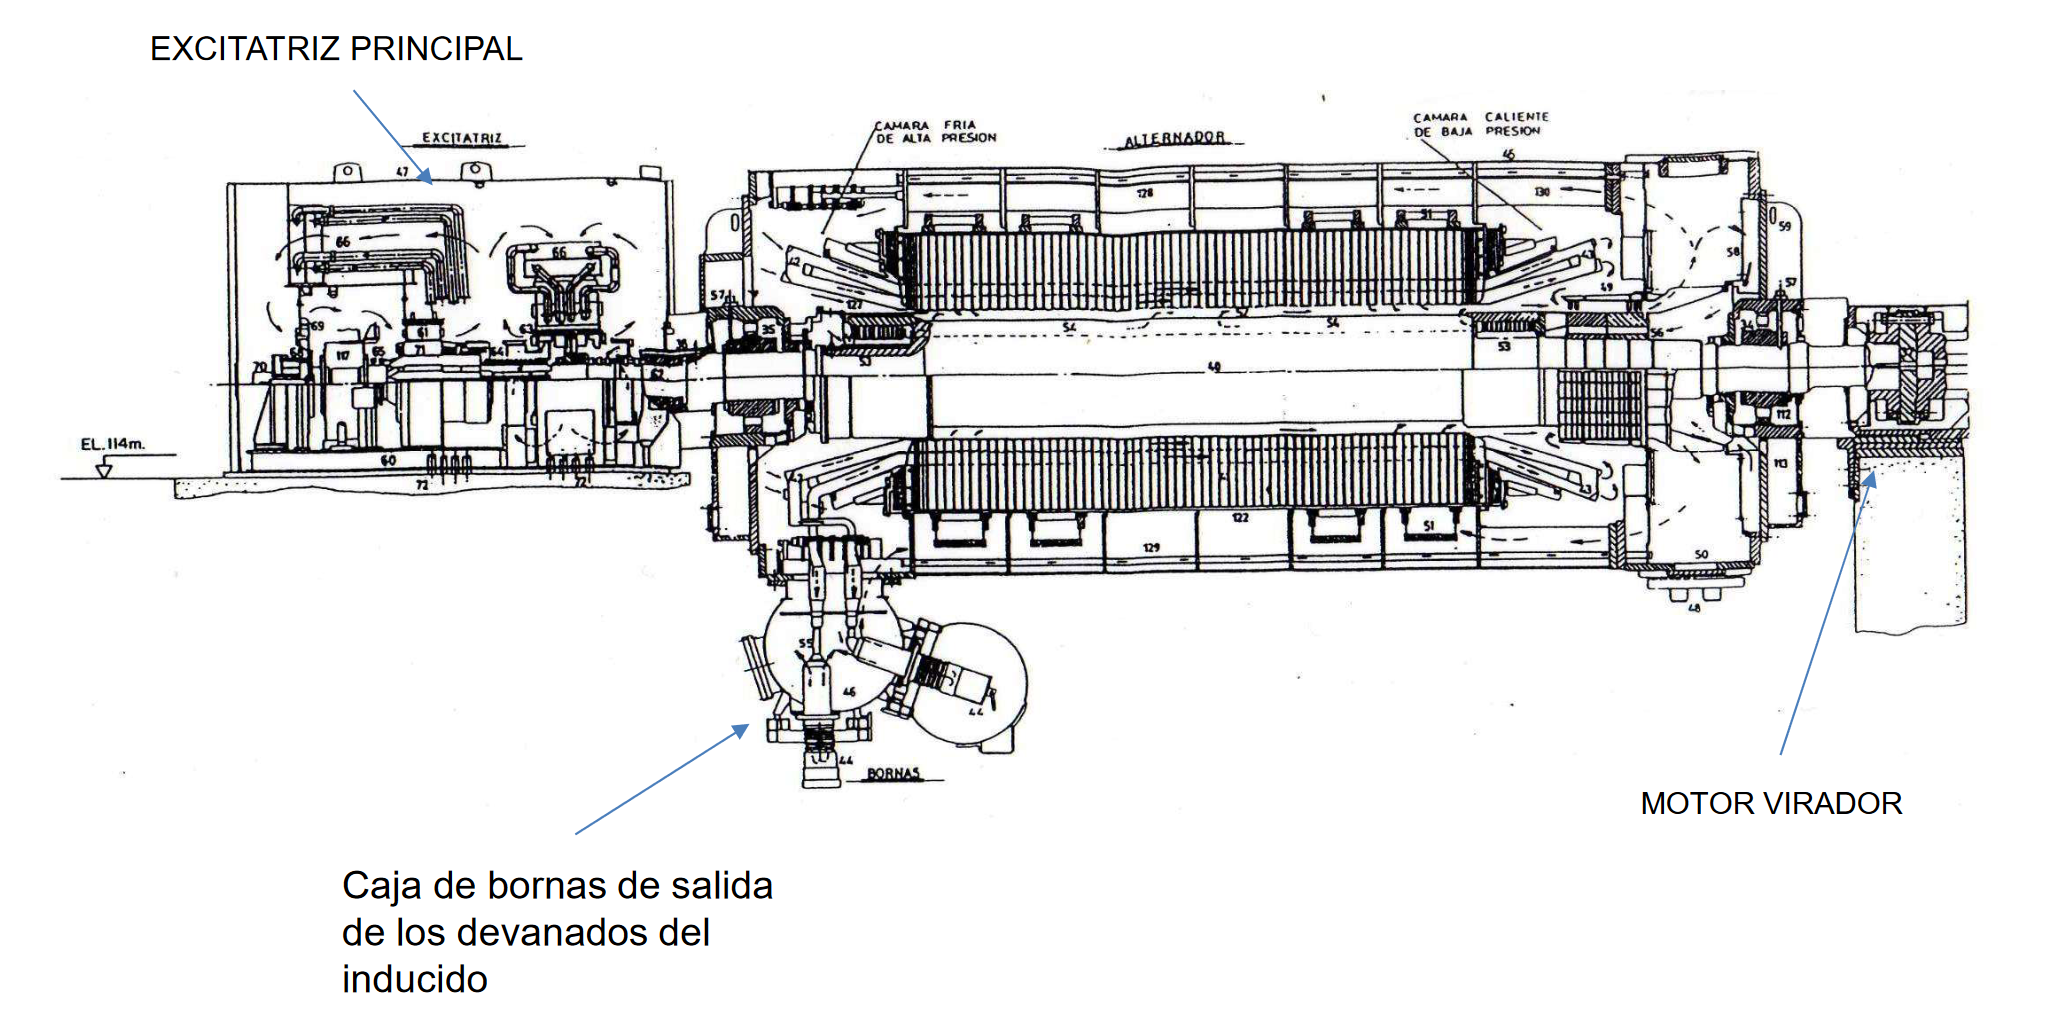
\includegraphics[width=1\linewidth]{res/tema6/generador}
			\label{fig:generador}
		\end{figure}
		
		\subsection{Conductores de salida del estátor. Barras de fase aislada.}
			Tienen una capacidad nominal de corriente desde 3 $kA$ hasta 50 $kA$. Se prolongan hasta el bloque interruptor automático + seccionador, bornes de baja tensión del transformador de potencia y el lado
			de alta tensión del transformador de servicios auxiliares. Por su interior circula aire o hidrógeno mediante ventiladores centrífugos. Consta de las siguientes partes:
			
			\begin{itemize}
				\item \textbf{Conductor:} puede ser un tubo redondo de aluminio extruido de alta conductividad o barras de cobre.
				\item \textbf{Aisladores:} pueden ser de porcelana o de resina epoxy. Están sujetos rígidamente a los tubos de aluminio. Puede haber de uno a cuatro aisladores.
				\item \textbf{Tubo pantalla:} Es de aluminio. Su misión es doble: servir como conducto para la circulación del refrigerante (hidrógeno o aire) y como apantallamiento para el flujo creado por las altas intensidades. Se ponen a tierra por varios puntos.
			\end{itemize}
		
		\subsection{Circuito equivalente por fase de un generador síncrono.}
			\subsubsection{Principio de funcionamiento.}
				En una máquina síncrona las tensiones inducidas forman un sistema trifásico equilibrado y de secuencia directa. Estas tensiones inducidas, si no se consideran efectos de saturación, son proporcionales a la intensidad de excitación en corriente continua, dado que la velocidad de rotación tiene que ser constante para mantener la frecuencia de la red constante.
				
				
				\begin{figure}[H]
					\begin{minipage}{0.5\textwidth}
						\begin{figure}[H]
							\centering
							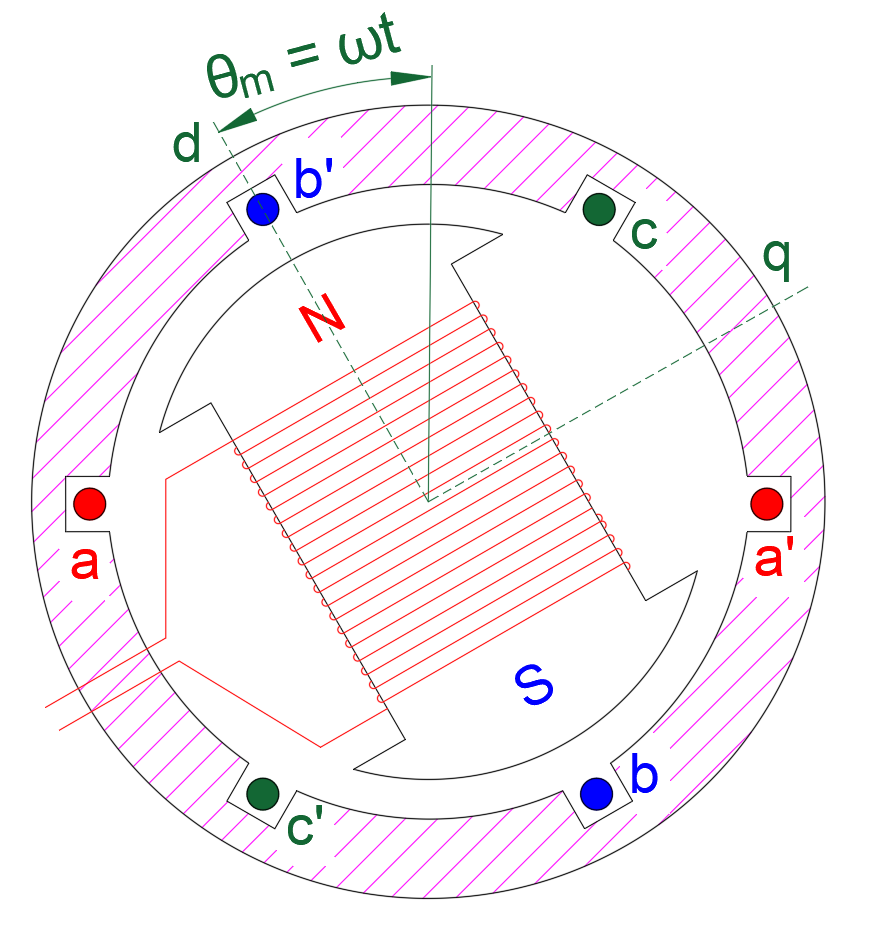
\includegraphics[width=0.7\linewidth]{res/tema6/ejes_dq}
							\label{fig:ejesdq}
						\end{figure}
					\end{minipage}
					\begin{minipage}{0.5\textwidth}
						Si el generador es de polos salientes la reluctancia en el entrehierro no es uniforme y aparecen dos reactancias:
						\begin{itemize}
							\item \textbf{Reactancia del eje directo:} $X_d$.
							\item \textbf{Reactancia del eje transversal o en cuadratura:} $X_q$.
						\end{itemize}
						Si el generador es de rotor cilíndrico sólo se considera la \textbf{reactancia síncrona:} $X_s$.
						
						\[f = \dfrac{p\cdot n}{60} \qquad E = k\cdot \omega \cdot i_{ex}\]
					\end{minipage}
				\end{figure}
			
			\subsubsection{Circuito equivalente por fase.}
				Considerando un generador de rotor cilíndrico o liso, al conectarla una carga y circular intensidad, estas corrientes crean un campo magnético, denominado \textbf{reacción de inducido}, que presenta una distribución senoidal y que gira a la misma velocidad y en el mismo sentido que el rotor. Esto provoca una caída de tensión en carga respecto de la tensión en vacío, y se representa mediante una reactancia de reacción de inducido, $X_{ri}$.
				
				
				No todo el flujo que crea el inductor es recogido por el inducido. Esta pérdida de flujo se representa mediante una reactancia de dispersión $X_\sigma$.
				
				\begin{figure}[H]
					\centering
						\begin{circuitikz}
							\tikzstyle{every node}=[font=\normalsize]
							\draw (3.25,18) to[sinusoidal voltage source, sources/symbol/rotate=auto,l={$\vec E_a$}] (3.25,14.75);
							\draw (3.25,18) to[L,l={$jX_{ri}$} ] (5,18);
							\draw (5,18) to[L,l={$jX_\sigma$} ] (6.75,18);
							\draw (6.75,18) to[R,l={$R$}] (8.5,18);
							\draw [](8.5,18) to[short, -o] (9,18) ;
							\draw [](3.25,14.75) to[short, -o] (9,14.75);
							\draw [->, >=Stealth] (9,17.5) -- (9,15.25)node[pos=0.5,right, fill=white]{$\vec U_a$};
							\draw [short] (3.5,19) -- (6.5,19)node[pos=0.5,above, fill=white]{$jX_s$};
							\draw [short] (3.5,19) -- (3.5,18.75);
							\draw [short] (6.5,19) -- (6.5,18.75);
							\draw [->, >=Stealth] (8.25,18) -- (8.75,18)node[pos=0.7,above]{$\vec I_a$};
							\draw [->, >=Stealth] (5,17.5) -- (5,15.25)node[pos=0.5,right]{$\vec E_{ag}$};
						\end{circuitikz}
				\end{figure}
				
				\begin{figure}[H]
					\centering
					\begin{circuitikz}
						\tikzstyle{every node}=[font=\normalsize]
						\draw [ color={rgb,255:red,0; green,0; blue,255}, ->, >=Stealth] (5,14.75) -- (7.75,14.75)node[pos=1,above]{$\vec{U}$};
						\draw [ color={rgb,255:red,255; green,0; blue,0}, ->, >=Stealth] (7.75,14.75) -- (8.5,14)node[pos=1,below]{$R\vec{I}$};
						\draw [ color={rgb,255:red,255; green,0; blue,0}, ->, >=Stealth] (8.5,14) -- (10.5,16.25)node[pos=0.5,right]{$jX_\sigma\vec{I}$};
						\draw [ color={rgb,255:red,0; green,128; blue,0}, ->, >=Stealth] (5,14.75) -- (10.5,16.25)node[pos=0.9,above]{$\vec{E}_{ag}$};
						\draw [ color={rgb,255:red,128; green,0; blue,255}, ->, >=Stealth] (5,14.75) -- (6.5,13.25)node[pos=1,below]{$\vec{I}$};
						\draw [ color={rgb,255:red,210; green,105; blue,0}, ->, >=Stealth] (5,14.75) -- (4,17.75)node[pos=1,right]{$\Phi$};
						\draw [ color={rgb,255:red,255; green,128; blue,0}, ->, >=Stealth] (5,14.75) -- (4.25,17)node[pos=1,right]{$\vec{F}_{r}$};
						\draw [ color={rgb,255:red,255; green,0; blue,128}, ->, >=Stealth] (4.25,17) -- (3,18.25)node[pos=0.8,above]{$\,\,\,\,\vec{F}_i$};
						\draw [ color={rgb,255:red,0; green,128; blue,128}, ->, >=Stealth] (5,14.75) -- (11.75,17.75)node[pos=0.9,above]{$\vec{E}_a$};
						\draw [ color={rgb,255:red,255; green,0; blue,0}, ->, >=Stealth] (10.5,16.25) -- (11.75,17.75)node[pos=0.5,right]{$jX_r\vec{I}$};
						\draw [ color={rgb,255:red,128; green,128; blue,128}, ->, >=Stealth] (5,14.75) -- (2.425,19.25)node[pos=1,left]{$\Phi_0$};
						\draw [->, >=Stealth] (5,14.75) -- (3,18.25)node[pos=0.9,left]{$\vec{F}_{ex}$};
						\draw (6,14.75) arc [radius=1cm, start angle=0, end angle=-45]node[pos=0.6,right]{$\varphi$};
						\draw (6.5,14.75) arc [radius=1.5cm, start angle=0, end angle=25]node[pos=0.4,right]{$\delta$};
						\draw (7,15.275) arc [radius=2cm, start angle=10, end angle=19]node[pos=0.9,right]{$\delta_m$};
					\end{circuitikz}
				\end{figure}